\chapter{Kappa Language Extensions}

Note on terminology. In the following 'voxel' means a subunit of a defined compartment. Species is mostly used to refer to a particular agent or complex in the model.

\section{Existing Kappa language}

The current Kappa language consists of the following constructs, as described in the KaSim 2.01 documentation \citep{KaSimManual2012}. A more formal description of the language grammar (including the spatial extensions) is given in Appendix \ref{chap:spatialGrammar}.

\bigskip 
\textbf{Comments}:

\begin{kappasource}
# This is a comment
\end{kappasource} 

\textbf{Agents}:

\begin{kappasource}
AgentName
AgentName()
AgentName(stateWithValue~stateValue, stateWithNoValue, unboundSite, boundSite!1)
\end{kappasource} 


\textbf{Non-spatial transition rules}:

\begin{kappasource}
'state change' A(state~old) -> A(state~new) @ 0.1
'binding'      A(bindsite),B(bindsite) -> A(bindsite!1),B(bindsite!1) @ 0.1
'unbinding'    A(bindsite!1),B(bindsite!1) -> A(bindsite),B(bindsite) @ 0.1
'creation'     -> A() @ 0.1
'degradation'  A() -> @ 0.1
A(state~old) -> A(state~new) @ 0.1 # Unnamed transform rule
\end{kappasource} 

\textbf{Initial species values}:

\begin{kappasource}
\%init 1000 A(state~old),C()            # 1000 of each of A(..) and C()
\%init 2000 A(bindsite!1),B(bindsite!1) # 2000 of the bound complex A(..),B(..)
\end{kappasource} 

\textbf{Observables and named variables}: Variables can be referenced in perturbation calculations, but do not show in outputs as observations.

\begin{kappasource}
\%obs 'Label' A()  # All agents A()
\%obs A()          # Unnamed observation, will default to 'A()' in outputs
\%obs A(state~old) # All agents matching A(state~old)
\%obs 'binding'    # Activity of the transform rule named 'binding'

\%var 'Named variable' B()
\end{kappasource} 



\section{Concepts to encapsulate}

The spatial Kappa language requires some encoding of the following concepts to be useful.

\begin{itemize}
 \item A description of \textbf{compartments} and their \textbf{dimensions}. A model may have multiple compartments each containing reacting species. The dimensions are necessary to define the shape of a compartment, be it a single cell, a 1 dimensional linear array of voxels, a 2 dimensional grid of some form, or a 3 dimensional lattice structure. Relative differences in size of different compartments can be specified, e.g. the reacting volume of a nucleus relative to the surrounding cytosol. Relative differences in shape can also be specified, for example the thin layer of cytosol next to the inner surface of the plasma membrane versus the rest of the cytosol.

 \item Predefined compartment shapes. To concisely create more accurate models, predefined compartment shapes in 2 and 3 dimensions can be chosen, these include open and closed circles, spheres and cylinders. 

 \item A description of \textbf{channels}, both intra-compartment and inter-compartment. The intra-compartment channel specification should be rich enough to allow description of multiple structures, e.g. in 1D linear arrays or circles, in 2D square or hexagonal meshes, cylinders or tori, in 3D cubes, filled cylinders, spheres, etc.

 \item Predefined channels. Commonly used inter and intra-compartment channels can be easily specified by name.

 \item A means of \textbf{locating species} within compartments, e.g. all DNA would reside within the nucleus, or cell receptors would be limited to the plasma membrane. Note that a multi-agent species need not be confined to a single voxel, but may span neighbouring, connected voxels.

 \item A means of \textbf{locating transition rules} within compartments, e.g. DNA transcription is isolated to the nucleus. The language should also allow the same transform rule to be specified with different rates depending on the location of the reacting species.

 \item A description of the \textbf{transport} (active or diffusive) of species within a compartment or between compartments along previously described channel structures. The rates of transport should be general to all species, or species specific. Note that transport of multi-voxel species should also be possible.

\end{itemize}


\textbf{Additional concepts}

\begin{itemize}
 \item \textbf{Granularity} within compartments. It would be useful to be able to specify locations at the level of compartments or single voxels within a compartment. This would allow the model to represent, for example, a signal cascade being initiated as one point in the cytosol, and the resulting signal molecules being diffused through the cytosol. 

 \item \textbf{Backwards compatibility} with basic Kappa. Given the quantity of existing models, the extended language should allow the existing models to work as before without modification. The user should have the choice of not using the spatial aspects of the extended language with no rework penalty.

\end{itemize}


\section{New language constructs}

A full BNF description of the extended Kappa grammar is given in Appendix \ref{chap:spatialGrammar}. The new constructs are identifiable as new rule types (\verb|%channel| and \verb|%compartment|), and location or channel identifiers in existing rule types prefixed with `\verb|:|'.

\subsection{Compartments and voxels}

Compartments are defined as single voxels or regular multidimensional arrays of voxels as follows
\begin{bnfsource}
'\%compartment:' name=id ('[' INT ']')*
\end{bnfsource}
For example
\begin{kappasource}
\%compartment: SingleCell 
\%compartment: 1dArray' [10]       # 10 voxels in size 
\%compartment: 2dArray' [10][5]    # 10x5 voxels in size 
\%compartment: 3dArray' [10][5][4] # 10x5x4 voxels in size 
\end{kappasource}

Compartments or individual voxels within a compartment can be referenced using the following location syntax
\begin{bnfsource}
':' id ( '[' cellIndexExpr ']' )*
\end{bnfsource}
where
\begin{bnfsource}
cellIndexExpr :
  cellIndexAtom operator_cell_index cellIndexAtom
  | cellIndexAtom
  
cellIndexAtom :
  '(' cellIndexExpr ')'
  | INT
  | id
  
operator_cell_index :
  '+' | '-' | '*' | '/' | '\%'
\end{bnfsource}
For example
\begin{kappasource}
:myCompartment                     # the compartment as a whole
:myCompartment [0][0][0]           # the first voxel in a 3d array compartment
:myCompartment [4]                 # the fifth voxel in a 1d linear arrays

:myCompartment [x][y][z]           # variable name usage described in
:myCompartment [x*2][y -1][z+(x*3)] #   channel section below
\end{kappasource}

In all situations where locations are used, it is only legal to refer to the compartment as a whole by omitting the cell indices, or refer to a single voxel, by fully defining the correct number of cell indices to match the dimensions of the compartment. Also, variable names are only permitted in locations within channel definitions, described below.

\subsubsection{Predefined compartment types}

Commonly used non-rectangular compartments can also be concisely defined. These include both solid and hollow (open) shapes in 2 and 3 dimensions. The available predefined compartment types are

\medskip 

\begin{tabular}{|c|cccc|}
\hline
Name & \multicolumn{4}{|c|}{Parameters}\\ 
\hline
\multicolumn{5}{|c|}{2D}\\
\hline
OpenRectangle & height & width & thickness & \\
SolidCircle & diameter &  &  & \\
OpenCircle & diameter & thickness &  & \\
\hline
\multicolumn{5}{|c|}{3D}\\
\hline
OpenCuboid & height & width & depth & thickness\\
SolidSphere & diameter &  &  &  \\
OpenSphere & diameter & thickness &  & \\
SolidCylinder & diameter & length & & \\
OpenCylinder & diameter & length & thickness & \\
\hline
\end{tabular} 

\medskip 

This allows the creation of a voxellated approximation of the shape specified, which can then be used for simulation. For the open compartment types, thickness specifies how thick in voxels the compartment reaction volume is.

\begin{figure}[h!]
 \centering
 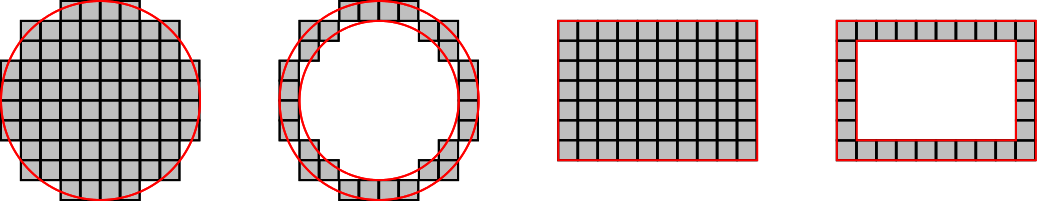
\includegraphics[scale=0.2]{./images/compartmentTypes.png}
 % compartmentTypes.png: 1042x202 pixel, 51dpi, 52.10x10.10 cm, bb=0 0 1477 286
 \caption{2D compartment types (open and solid)}
 \label{fig:compartmentTypes}
\end{figure}



The syntax to specify these compartments is
\begin{bnfsource}
'\%compartment:' name=id type=id ('[' INT ']')*
\end{bnfsource}
For example
\begin{kappasource}
### 2D Shapes

%compartment: solidRectangle              [10][5]        # [height][width]
%compartment: openRectangle OpenRectangle [10][5] [2]    # [height][width] [thickness]
%compartment: solidCircle   SolidCircle   [10]           # [diameter]
%compartment: openCircle    OpenCircle    [10] [2]       # [diameter] [thickness]

### 3D Shapes

%compartment: solidCuboid                 [10][5][8]     # [height][width][depth]
%compartment: openCuboid    OpenCuboid    [10][5][8] [2] # [height][width][depth] [thickness]
%compartment: solidSphere   SolidSphere   [10]           # [diameter]
%compartment: openSphere    OpenSphere    [10] [2]       # [diameter] [thickness]
%compartment: solidCylinder SolidCylinder [10][8]        # [diameter][length]
%compartment: openCylinder  OpenCylinder  [10][8] [2]    # [diameter][length] [thickness]
\end{kappasource}



\subsection{Channels}

The structure of a compartment is further defined by how voxels within the compartment are linked to each other and to connected compartments. The channels are then used in defining both static links between agents, and movement of agents through the geometry of the model. These channels are defined as follows
\begin{bnfsource}
'\%channel:' id channel
| '\%channel:' id '(' channel ')' ('+' '(' channel ')')*
\end{bnfsource}
where
\begin{bnfsource}
channel :
  source=locations '->' target=locations

locations :
  location (',' location)*
\end{bnfsource}
Where \verb|location| is as described above. For example
\begin{kappasource}
\%compartment: 2dArray [10][200]    # 10x200 voxels in size 

# Link all voxels to their horizontally adjacent neighbours
# Link all voxels to their vertically adjacent neighbours
# Wrap around the voxels on the left and right edges to create a cylinder
# Wrap around the voxels on the top and bottom edges to create a torus
\%channel: meshlinks {\textbackslash}
    (:2dArray[x][y] -> :2dArray[x+1][y]) + (:2dArray[x][y] -> :2dArray[x -1][y]) +{\textbackslash}
    (:2dArray[x][y] -> :2dArray[x][y+1]) + (:2dArray[x][y] -> :2dArray[x][y -1]) +{\textbackslash}
    (:2dArray[0][y] -> :2dArray[9][y])   + (:2dArray[9][y] -> :2dArray[0][y]) +{\textbackslash}
    (:2dArray[x][0] -> :2dArray[x][199]) + (:2dArray[x][199] -> :2dArray[x][0])
\end{kappasource}

The above code defines a thin torus composed of a 2d mesh.

Locations on the left hand side of the channel definitions above may contain either constant values or single variable names, not complex expressions. The variable names are used to define the dimensions which will be iterated through to produce links. Locations on the right hand side allow constant values or complex expressions involving the variables defined on the left hand side of the expression. It is invalid for the right hand expression to use variables not defined on the left. If setting the values of variables references valid voxels on both the left and right, then those voxels are deemed to be linked. References which refer to voxels outside the dimensions of the compartment are ignored, and no link is created. The references in a channel expression can refer to the same compartment, or two different compartments. The modulus operator \verb|%| is useful in defining regular, repeating linkage patterns within the compartment, for example the 2D hexagonal mesh described in Appendix \ref{sec:spatialPatterns}.

Channels can make use of multiple source voxels simultaneously. For example if a model was to represent the movement of transmembrane proteins laterally along the surface of a membrane, then the channel used to describe the lateral motion would need to include simultaneous movement in two compartments (cytosol and membrane). This is represented as follows:

\begin{kappasource}
\%compartment: membrane [5][5]
\%compartment: cytosol [5][5][5]

\%channel: diffusion {\textbackslash}
    (:membrane [x][y], :cytosol [u][v][0] -> :membrane [x+1][y], :cytosol [u+1][v][0]) + {\textbackslash}
    (:membrane [x][y], :cytosol [u][v][0] -> :membrane [x -1][y], :cytosol [u -1][v][0]) + {\textbackslash}
    (:membrane [x][y], :cytosol [u][v][0] -> :membrane [x][y+1], :cytosol [u][v+1][0]) + {\textbackslash}
    (:membrane [x][y], :cytosol [u][v][0] -> :membrane [x][y -1], :cytosol [u][v -1][0])
\end{kappasource}

Here, variables x,y represent locations in the membrane, and u,v represent locations in the cytosol. The definition updates the locations in these two compartments in unison.

Further examples of compartment and channel specifications for common structures are given in Appendix
 \ref{sec:spatialPatterns}.

\subsubsection{Predefined channel types}

Commonly used 2D and 3D channel types can be concisely defined. 

\medskip 

\begin{tabular}{|c|l|}
\hline
Name & \multicolumn{1}{|c|}{Each voxel connected to}\\ 
\hline
\multicolumn{2}{|c|}{2D}\\
\hline
EdgeNeighbour & 4 neighbours which share an edge in grid \\
Hexagonal & 6 neighbours which share an edge in hexagonal grid \\
Neighbour & 8 neighbours which share an edge or corner in grid \\
\hline
\multicolumn{2}{|c|}{3D}\\
\hline
FaceNeighbour & 6 neighbours which share a face in grid\\
Neighbour & 26 neighbours which share a face, edge or corner in grid \\
\hline
\end{tabular} 

\medskip 

\begin{figure}[h!]
 \centering
 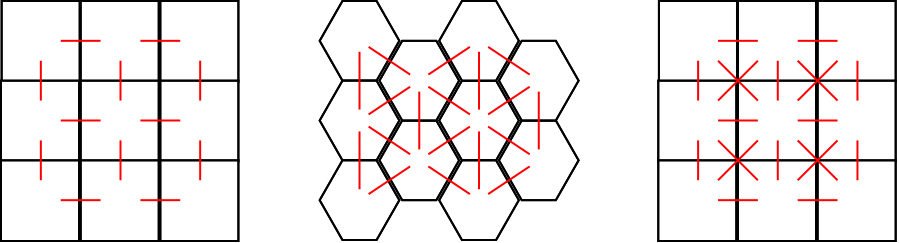
\includegraphics[scale=0.2]{./images/channelTypes.png}
 % channelTypes.png: 1042x202 pixel, 51dpi, 52.10x10.10 cm, bb=0 0 1477 286
 \caption{2D channel types: EdgeNeighbour, Hexagonal and Neighbour}
 \label{fig:channelTypes}
\end{figure}

There are also predefined directional channel types usable in both 2D and 3D compartments


%channel: radial Radial :solidRectangle -> :solidRectangle
%channel: radialIn RadialIn :solidRectangle -> :solidRectangle
%channel: radialOut RadialOut :solidRectangle -> :solidRectangle
%channel: lateral Lateral :solidRectangle -> :solidRectangle

\medskip 

\begin{tabular}{|c|l|}
\hline
Name & \multicolumn{1}{|c|}{Each voxel connected to}\\ 
\hline
Radial & neighbours both directly towards and away from compartment centre  \\
RadialIn & neighbours both directly towards compartment centre \\
RadialOut & neighbours both directly away from compartment centre \\
Lateral & neighbours at same distance from compartment centre \\
\hline
\end{tabular} 

\medskip 

\begin{figure}[h!]
 \centering
 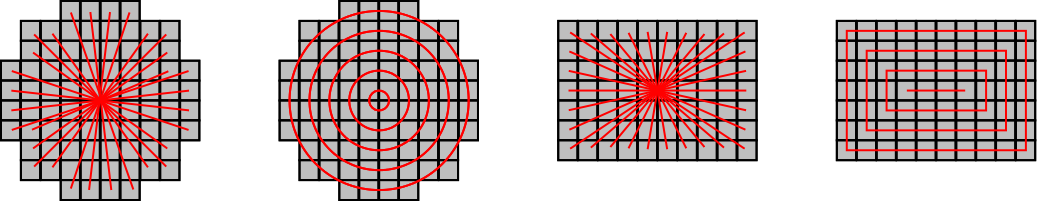
\includegraphics[scale=0.2]{./images/directedChannelTypes.png}
 % directedChannelTypes.png: 1042x202 pixel, 51dpi, 52.10x10.10 cm, bb=0 0 1477 286
 \caption{Directed channel types: Radial and Lateral}
 \label{fig:directedChannelTypes}
\end{figure}

The syntax to use a predefined channel type is

\begin{bnfsource}
'\%channel:' id channel
| '\%channel:' id '(' channel ')' ('+' '(' channel ')')*
\end{bnfsource}
where
\begin{bnfsource}
channel :
  type=id source=locations '->' target=locations
\end{bnfsource}
Where \verb|locations| is as described above. For example
\begin{kappasource}
\%compartment: 2dArray [10][200]    # 10x200 voxels in size 
\%compartment: solidRectangle[5][5] # [height][width]

\%channel: radial Radial :solidRectangle -> :solidRectangle
\%channel: radialIn RadialIn :solidRectangle -> :solidRectangle
\%channel: radialOut RadialOut :solidRectangle -> :solidRectangle
\%channel: lateral Lateral :solidRectangle -> :solidRectangle
\end{kappasource}

NOTE - these currently work only for intra-compartment channels

\subsection{Locating agents}

The definitions above can now be used to locate species within the model. Any rule that accepts a definition of agents (i.e. transition, var, obs, init rules), now allows these agents to be located. For each group of agents, a prefixed location constrains the agents to that location. For example

\begin{kappasource}
\%compartment: membrane [5][5]
\%compartment: cytosol [5][5][5]

\%init: 1000 A                   # A distributed evenly among all voxels in model 
\%init: 1000 :cytosol B          # B distributed evenly among all voxels in cytosol
\%init: 1000 :membrane[2][2] C   # C in one voxel of the membrane only 
\end{kappasource}

In addition, individual agents can have a specified location. For example
\begin{kappasource}
\%init: 1000 B:cytosol             # B distributed evenly among all voxels in cytosol
\%init: 1000 C:membrane[2][2](s~u) # C in one voxel of the membrane only 
\end{kappasource}

When locations are specified both for agent groups and individual agents, the individual agent location takes precedence. This allows for concise definition of agent groups where all but one of the agents in the group share a location.

\subsection{Agent links}

Agents in neighbouring voxels linked by a defined channel can be linked together. This is an extension of the basic Kappa link syntax to name the channel used to link the agents. For example

\begin{kappasource}
\%compartment: membrane [5][5]
\%compartment: cytosol [5][5][5]

\%channel: domainLink {\textbackslash}
    (:membrane [x][y] -> :cytosol [x][y][0]) + (:cytosol [x][y][0] -> :membrane [x][y])

\%init: 1000 A:membrane(d!1:domainLink), B(d!1)
\end{kappasource}

The above describes a model where the species A-B exists in two compartments, B in the cytosol and A embedded in the membrane. When specifying agent links using channels, only one end of the link needs to specify the channel. If a link does not specify the channel, it is assumed that both agents party to the link exist in the same voxel.

Links including channels can be created or broken in the same way as basic Kappa links in transition rules.

\subsection{Species movement}

Species can move along defined channels. Species movement is described using the \verb|->:| operator.
\begin{bnfsource}
(source=location)? '->:' channelName=id (target=location)?
| (a=agentGroup)? '->:' channelName=id (b=agentGroup)?
\end{bnfsource}

Movement transition rules can either constrain the movement by species chosen, or by source location. For example

\begin{kappasource}
\%compartment: membrane [5][5]

\%channel: diffusion {\textbackslash}
    (:membrane [x][y] -> :membrane [x+1][y]) + (:membrane [x][y] -> :membrane [x - 1][y]) + {\textbackslash}
    (:membrane [x][y] -> :membrane [x][y+1]) + (:membrane [x][y] -> :membrane [x][y - 1])

'diffusion A' A(s,t) ->:diffusion A(s,t) @ 1.0
'diffusion B' B(s,t) ->:diffusion B(s,t) @ 1.0
'diffusion AB' A(s!1,t),B(s!1,t) ->:diffusion A(s!1,t),B(s!1,t) @ 0.5

'diffusion all' ->:diffusion @ 1.0 # All species located in a single voxel will match this rule
\end{kappasource}

To describe movement of species which span more than one voxel, use the multi agent channel definition above. For example

\begin{kappasource}
\%compartment: membrane [5][5]
\%compartment: cytosol [5][5][5]

\%channel: diffusion {\textbackslash}
    (:membrane [x][y], :cytosol [u][v][0] -> :membrane [x+1][y], :cytosol [u+1][v][0]) + {\textbackslash}
    (:membrane [x][y], :cytosol [u][v][0] -> :membrane [x -1][y], :cytosol [u -1][v][0]) + {\textbackslash}
    (:membrane [x][y], :cytosol [u][v][0] -> :membrane [x][y+1], :cytosol [u][v+1][0]) + {\textbackslash}
    (:membrane [x][y], :cytosol [u][v][0] -> :membrane [x][y -1], :cytosol [u][v -1][0])

\%channel: domainLink {\textbackslash}
    (:membrane [x][y] -> :cytosol [x][y][0]) + (:cytosol [x][y][0] -> :membrane [x][y])

'diffusion A' A_m:membrane(s,t,d!1:domainLink),A_c(d!1) ->:diffusion {\textbackslash}
              A_m:membrane(s,t,d!1:domainLink),A_c(d!1) @ 1.0
'diffusion B' B_m:membrane(s,t,d!1:domainLink),B_c(d!1) ->:diffusion {\textbackslash}
              B_m:membrane(s,t,d!1:domainLink),B_c(d!1) @ 1.0

'diffusion AB' A_m:membrane(s!2,t,d!1:domainLink),A_c(d!1), {\textbackslash}
               B_m:membrane(s!2,t,d!3:domainLink),B_c(d!3) ->:diffusion {\textbackslash}
               A_m:membrane(s!2,t,d!1:domainLink),A_c(d!1), {\textbackslash}
               B_m:membrane(s!2,t,d!3:domainLink),B_c(d!3) @ 0.5
\end{kappasource}


\bigskip For example models demonstrating the use of the language extensions, refer to Appendix \ref{chap:resources}.

\newpage
